\chapter{État de l'art}

\section{Travaux existants}

À la connaissance de l’auteur, il n’existe pas de solution industrielle standardisée permettant de mesurer uniquement une portion de la réserve de marche par dévidage contrôlé du barillet, comme envisagé dans le cadre de ce projet. La solution proposée s’inscrit donc dans une démarche d’innovation visant à réduire le temps de mesure tout en conservant une information pertinente sur la réserve de marche du mouvement.

\section{Technologies et méthodes existantes}

Plusieurs technologies et méthodes existent pour automatiser la mesure de la réserve de marche ainsi que la détection de l’arrêt d’un mouvement horloger. Ces solutions peuvent être regroupées selon leur fonction principale au sein du système : la détection du fonctionnement du mouvement, le remontage automatisé et le contrôle du dévidage du barillet.

\subsection{Méthodes de détection du fonctionnement du mouvement}

La détection de l’état de fonctionnement (marche ou arrêt) du mouvement est une étape clé pour mesurer automatiquement la réserve de marche. Plusieurs approches sont utilisées dans l’industrie et la recherche :

\begin{itemize}
    \item \textbf{Détection acoustique} :  
    L’analyse du bruit de fonctionnement du mouvement (tic-tac) permet d’identifier la présence ou l’absence d’activité mécanique. L’arrêt du mécanisme se traduit par la disparition du signal acoustique périodique. Cette méthode est non intrusive et simple à mettre en œuvre, mais elle peut être sensible au bruit ambiant et nécessite un environnement relativement contrôlé.

    \item \textbf{Détection optique} :  
    La prise d’images ou de vidéos à intervalles réguliers permet d’observer le déplacement des aiguilles ou d’éléments mobiles du mouvement. L’absence de variation entre deux images successives indique l’arrêt du mécanisme. Cette approche est robuste et visuelle, mais elle implique un positionnement précis de la caméra, un éclairage constant et un traitement d’image pouvant être complexe.

    \item \textbf{Détection par vibrations} :  
    Des capteurs piézoélectriques ou des accéléromètres permettent de mesurer les micro-vibrations générées par le fonctionnement du mouvement. Lorsque la montre s’arrête, ces vibrations disparaissent. Cette méthode est relativement compacte et peu intrusive, mais peut nécessiter un filtrage du signal afin de distinguer les vibrations du mouvement de celles dues à l’environnement.

    \item \textbf{Méthodes hybrides} :  
    Certaines solutions combinent plusieurs types de capteurs (acoustique et vibration, par exemple) afin d’augmenter la fiabilité de la détection et de réduire les faux positifs liés au bruit ou aux perturbations externes.
\end{itemize}

\subsection{Méthodes de remontage automatisé du mouvement}

Pour garantir des conditions de test reproductibles, le remontage du mouvement peut être automatisé à l’aide de différents dispositifs :

\begin{itemize}
    \item \textbf{Systèmes de remontage motorisés par la tige de remontoir} :  
    Un moteur entraîne directement la tige de remontoir afin de simuler l’action manuelle de l’utilisateur. Cette solution permet de contrôler précisément le nombre de tours appliqués et de standardiser le niveau de remontage initial.

    \item \textbf{Simulation de la masse oscillante} :  
    Pour les mouvements automatiques, certains dispositifs reproduisent le mouvement du poignet afin de mettre en rotation la masse oscillante. Cette approche est représentative de l’usage réel, mais elle est plus complexe à mettre en œuvre et moins précise en termes de contrôle du nombre de tours effectivement transmis au barillet.

\end{itemize}

\subsection{Méthodes de contrôle du dévidage du barillet}

Le dévidage contrôlé du barillet permet de mesurer la réserve de marche ou d’étudier le comportement du mouvement en fonction de l’état de tension du ressort. Plusieurs technologies sont utilisées pour assurer ce contrôle :

\begin{itemize}
    \item \textbf{Motorisation par moteur pas à pas} :  
    Les moteurs pas à pas permettent de contrôler précisément le nombre de tours appliqués à la tige de remontoir ou à un mécanisme intermédiaire. Cette solution offre une bonne répétabilité et un contrôle précis de la position angulaire, ce qui est particulièrement adapté pour des mesures quantitatives de réserve de marche.

    \item \textbf{Motorisation par servomoteur} :  
    Les servomoteurs permettent un contrôle en position ou en vitesse, avec un retour d’information intégré. Ils sont simples à piloter, mais leur précision angulaire dépend fortement de la résolution de l’encodeur et de la qualité de l’asservissement.

    \item \textbf{Systèmes mécaniques à couple contrôlé} :  
    Certains dispositifs utilisent des limiteurs de couple ou des mécanismes à ressort afin de reproduire un dévidage progressif et maîtrisé. Ces solutions sont robustes, mais offrent généralement moins de flexibilité que les solutions motorisées pilotées électroniquement.
\end{itemize}
\section{Solutions industrielles existantes}
\subsection{Chronoscope RDM}

Le Chronoscope RDM (Réserve De Marche) de Witschi Electronic est une solution commerciale dédiée à la mesure automatique et contrôlée de la réserve de marche des mouvements et montres mécaniques. Cet appareil représente l'état de l'art en matière de test automatisé de réserve de marche dans l'industrie horlogère.

\subsubsection{Caractéristiques et principes de fonctionnement}

Le Chronoscope RDM effectue un test entièrement automatique permettant de mesurer la réserve de marche d'un mouvement avec une précision à la minute près \cite{Witschi_Chronoscope_RDM}. Le système embarque un écran tactile résistif de 4,3 pouces offrant une interface utilisateur claire, avec affichage en temps réel de l'avancement du test et des résultats. L'appareil peut mesurer des réserves de marche jusqu'à 999 heures sans intervention manuelle, ce qui en fait une solution particulièrement adaptée aux mouvements à longue autonomie.

Une caractéristique notable du Chronoscope RDM est son design empilable, qui permet de tester plusieurs mouvements simultanément tout en minimisant l'encombrement horizontal. De plus, l'appareil offre une grande flexibilité opérationnelle : les mouvements qui n'atteignent pas la réserve de marche attendue peuvent être retirés en cours de test sans interrompre l'évaluation des autres montres. Cette fonctionnalité est particulièrement utile en contexte de production ou de contrôle qualité, où les cadences de travail sont élevées.

\begin{figure}[H]
    \centering
    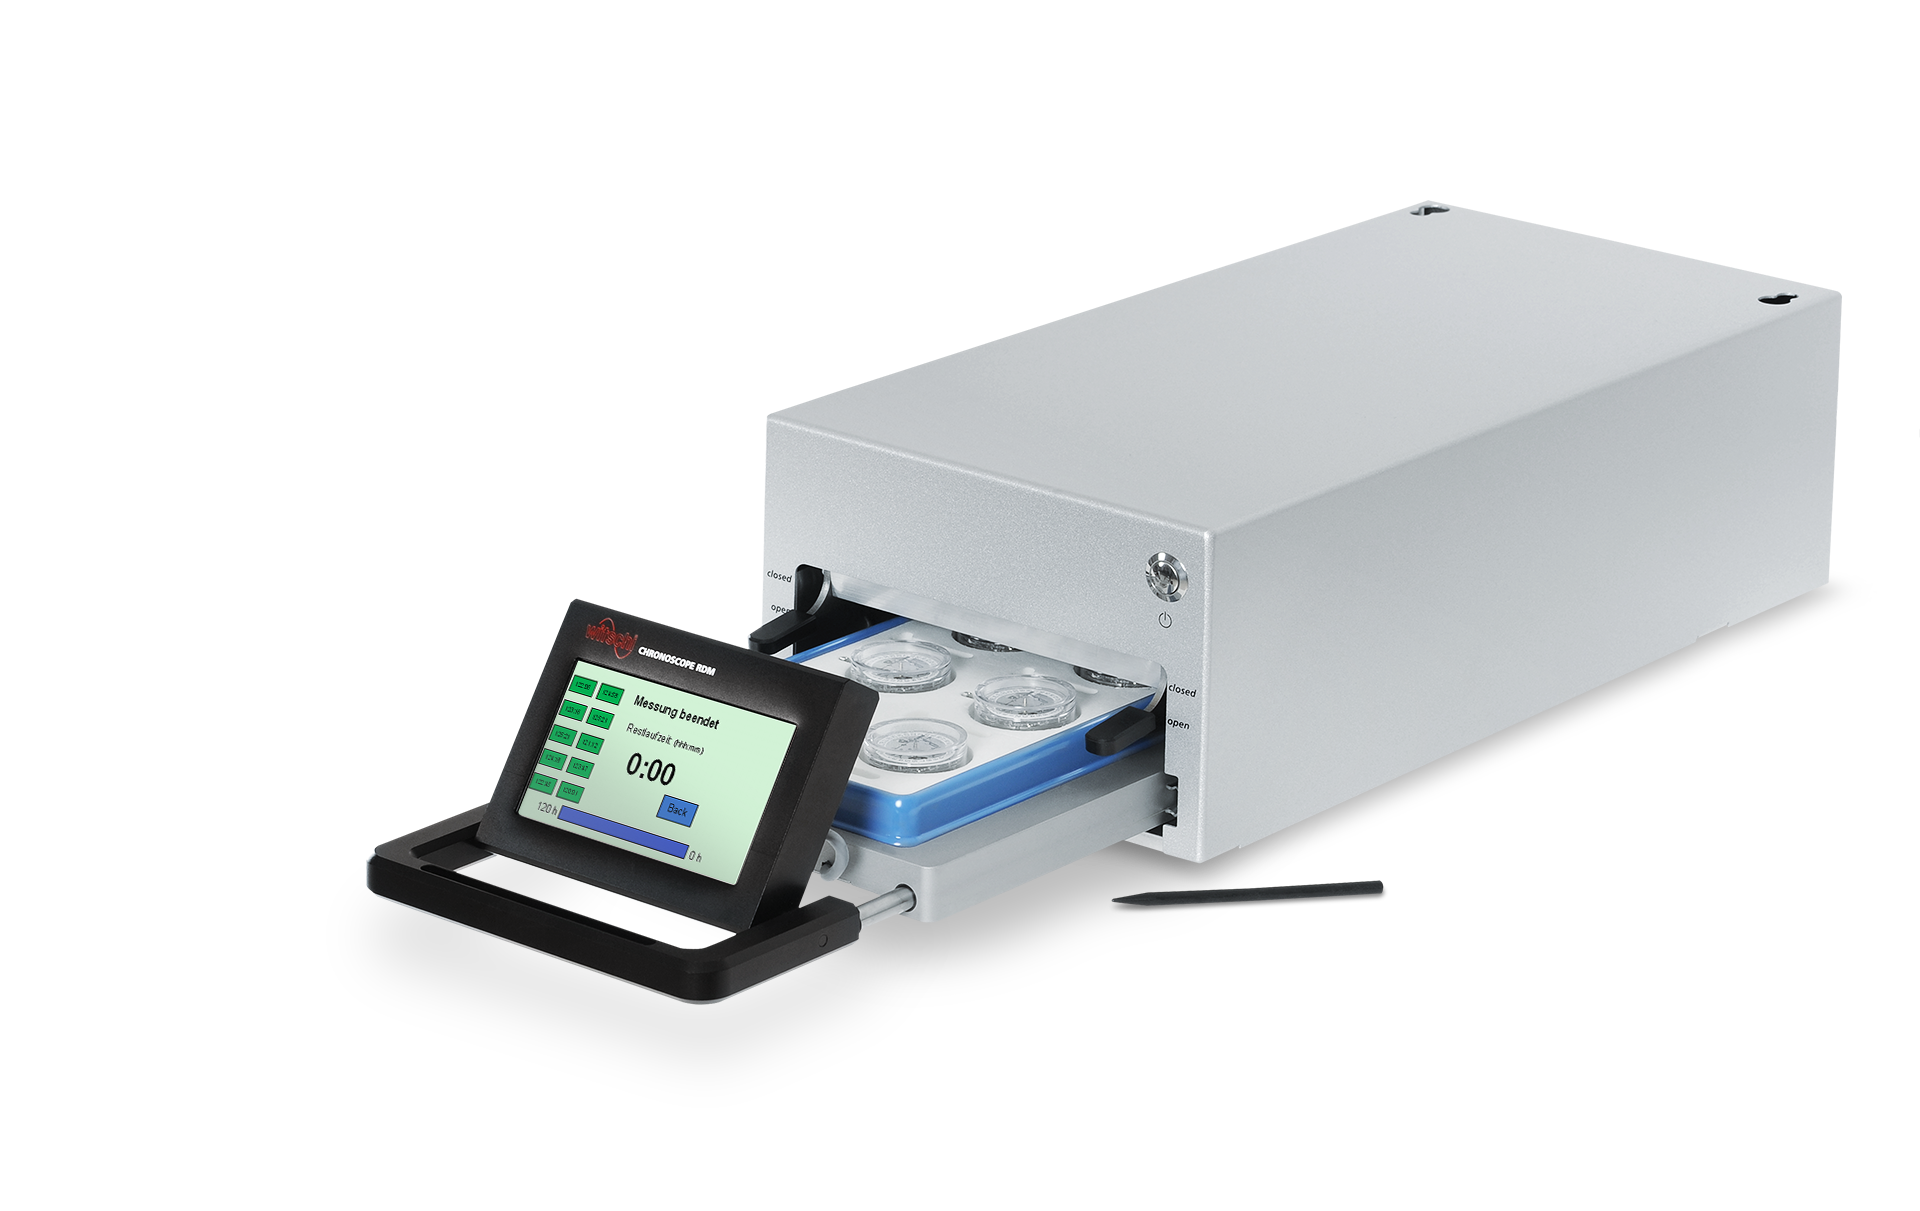
\includegraphics[width=0.45\textwidth]{assets/figures/Etat de l'art/MachineRM_Witschi_1.png}
    \hfill
    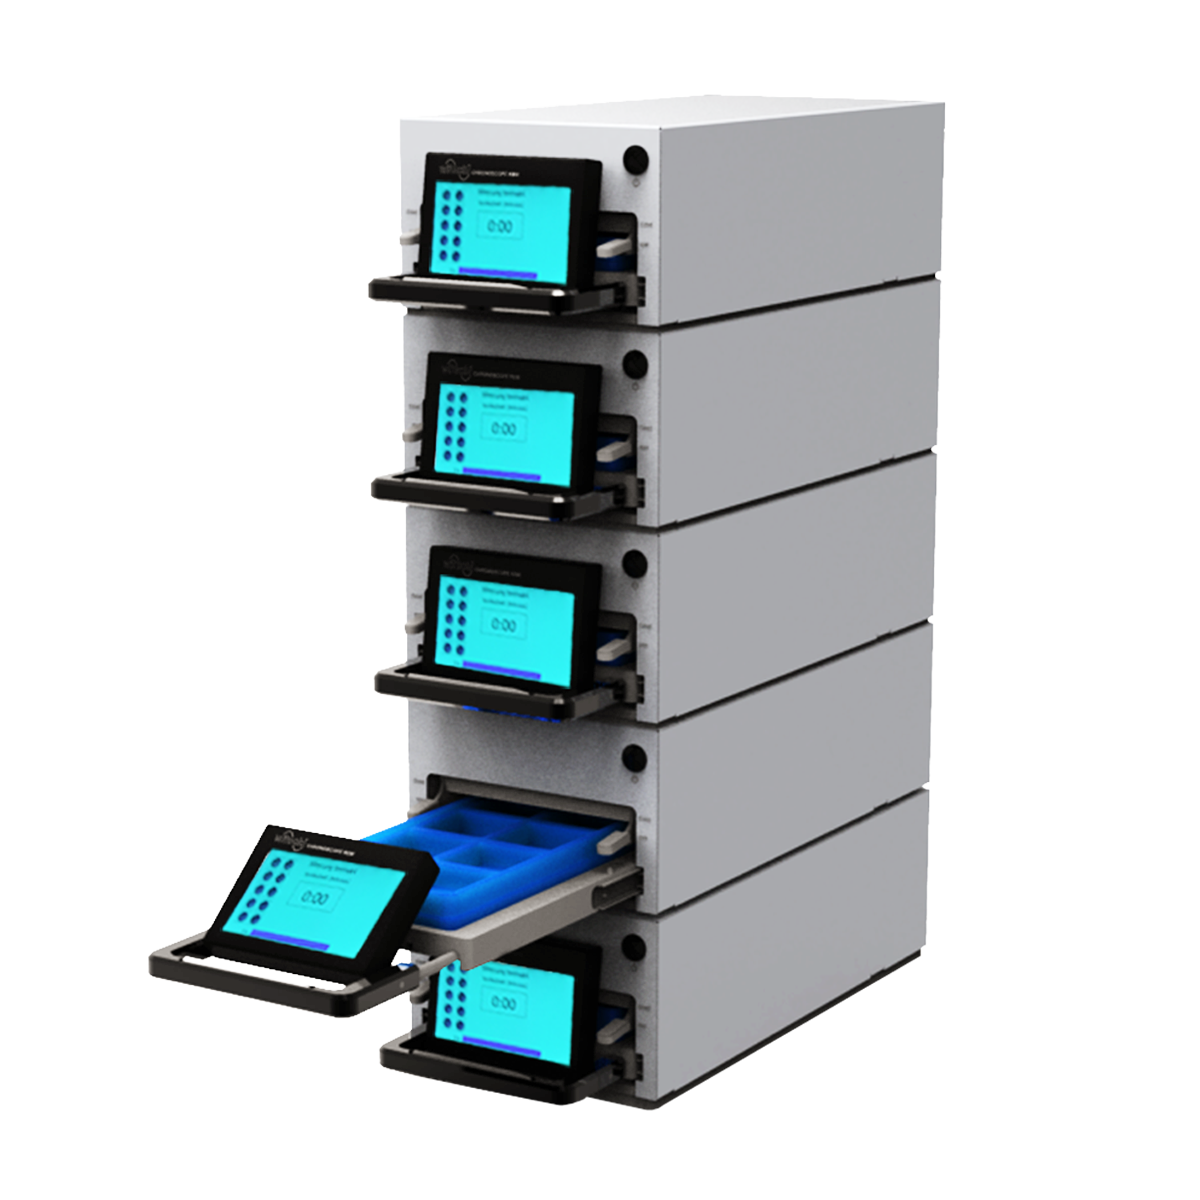
\includegraphics[width=0.45\textwidth]{assets/figures/Etat de l'art/MachineRM_Witschi_2.png}
    \caption{Chronoscope RDM de Witschi Electronic \cite{Witschi_Chronoscope_RDM}}
    \label{fig:chronoscope_rdm}
\end{figure}

\subsubsection{Avantages}

Le Chronoscope RDM présente plusieurs avantages significatifs :

\begin{itemize}
    \item \textbf{Mesure compacte} : Le design empilable permet de tester jusqu'à 10 mouvements simultanément en minimisant l'espace occupé sur le plan de travail, ce qui est un atout majeur pour les laboratoires et les ateliers ayant une place limitée.
    
    \item \textbf{Compatibilité large} : L'appareil peut traiter jusqu'à 10 mouvements d'origines et de types différents, offrant ainsi une grande flexibilité pour les ateliers traitant une variété de montres et de mouvements.
    
    \item \textbf{Mesure contrôlée et précise} : La précision à la minute près et le contrôle automatisé du test garantissent des résultats reproductibles et fiables, essentiels pour le contrôle qualité industriel.
    
    \item \textbf{Autonomie opérationnelle} : Le système fonctionne de manière entièrement automatique, permettant aux opérateurs de relâcher les mouvements à la minute juste à n'importe quelle heure, y compris en dehors des heures de travail classiques.
\end{itemize}

\subsubsection{Inconvénients}

Malgré ses atouts, le Chronoscope RDM présente également certaines limitations :

\begin{itemize}
    \item \textbf{Attente de la réserve de marche complète} : L'appareil mesure la totalité de la réserve de marche du mouvement. Cela signifie que pour un mouvement avec une réserve de 80 heures, le test complet dure 80 heures, ce qui représente un temps d'immobilisation considérable. Cette contrainte rend impératif une planification minutieuse de la production et limite l'agilité des tests rapides.
    
    \item \textbf{Investissement initial important} : Comme solution commerciale de haut de gamme, cet équipement représente un coût d'acquisition significatif, pouvant être un frein pour les petits ateliers ou les laboratoires aux budgets limités.
\end{itemize}

Malgré ces limitations, le Chronoscope RDM reste une référence industrielle pour les entreprises et laboratoires ayant besoin d'une mesure complète et certifiée de la réserve de marche. La machine proposée dans ce travail s'inscrit comme une alternative ou un complément, notamment pour les applications nécessitant une mesure partielle ou accélérée de la réserve de marche.

\subsection{Chrono RMV d'Icoflex}

Le Chrono RMV (Réserve de Marche Vision) d'Icoflex est une solution innovante basée sur l'analyse vidéo pour mesurer la réserve de marche de plusieurs têtes de montre ou calibres en parallèle \cite{Icoflex_Chrono_RMV}. Cet appareil représente une approche différente du Chronoscope RDM, en privilégiant la détection optique et le traitement d'image pour l'automatisation de la mesure.

\subsubsection{Caractéristiques et principes de fonctionnement}

Le Chrono RMV utilise une méthode de mesure optique basée sur l'analyse vidéo pour déterminer l'état de fonctionnement des mouvements \cite{Icoflex_Chrono_RMV}. Le système est capable de tester simultanément un grand nombre de têtes de montre ou calibres dans une configuration typique de 20 positions, permettant ainsi une productivité accrue. L'appareil capture une photographie du calibre ou de la tête de montre au départ et à la fin de la réserve de marche, permettant une documentation précise du test.

Le système embarque une base de données interne dédiée à la gestion des calibres et des têtes de montre, facilitant le suivi des résultats et l'organisation des tests \cite{Icoflex_Chrono_RMV}. Les données collectées peuvent être exportées au format CSV ou directement intégrées dans une base de données externe, offrant une flexibilité maximale pour l'intégration avec les systèmes informatiques existants.

Le design du Chrono RMV privilégie la compacité et la modularité. L'appareil est empilable et modulable, permettant d'adapter la configuration à des barquettes existantes (configurations sur-mesure). Cette approche rend le système particulièrement attractif pour les ateliers ayant des contraintes spatiales ou des besoins spécifiques de positionnement des mouvements.

\begin{figure}[H]
    \centering
    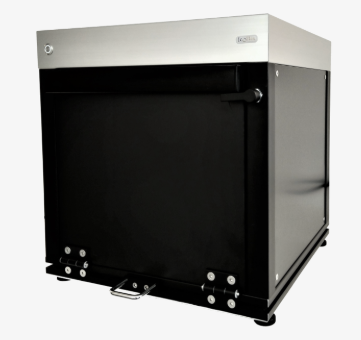
\includegraphics[width=0.75\textwidth]{assets/figures/Etat de l'art/ICOFLEX RMV.png}
    \caption{Chrono RMV d'Icoflex \cite{Icoflex_Chrono_RMV}}
    \label{fig:chrono_rmv_icoflex}
\end{figure}

\subsubsection{Avantages}

Le Chrono RMV présente plusieurs avantages distinctifs :

\begin{itemize}
    \item \textbf{Haute capacité de parallélisation} : Avec une configuration typique de 20 têtes de montre testées simultanément, le système offre une productivité significativement supérieure à celle du Chronoscope RDM, ce qui est idéal pour les environnements de production à fort volume.
    
    \item \textbf{Détection optique robuste} : La méthode de mesure par vision est non intrusive et permet une observation directe du comportement du mouvement sans contact mécanique, réduisant ainsi le risque d'endommagement ou d'influence sur le test.
    
    \item \textbf{Modularité et adaptabilité} : Le caractère modulable et la possibilité d'adapter le système à des barquettes existantes en font une solution flexible capable de s'intégrer dans des environnements de travail variés.
    
    \item \textbf{Gestion intégrée des données} : La base de données interne et la possibilité d'exporter les résultats au format CSV ou vers des systèmes externes facilitent le suivi et l'exploitation des données de test à long terme.
    
    \item \textbf{Design compact et empilable} : L'architecture empilable minimise l'encombrement au sol, ce qui est un atout majeur pour optimiser l'utilisation de l'espace dans les ateliers.
\end{itemize}

\subsubsection{Inconvénients}

Le Chrono RMV présente toutefois certaines limitations :

\begin{itemize}
    \item \textbf{Attente de la réserve de marche complète} : Tout comme le Chronoscope RDM, ce système mesure la totalité de la réserve de marche du mouvement. Cela implique des durées de test potentiellement très longues (jusqu'à plusieurs jours pour les mouvements à longue autonomie), ce qui représente une contrainte opérationnelle majeure.
    
    \item \textbf{Dépendance aux conditions d'éclairage et de vision} : La détection par analyse vidéo nécessite un éclairage constant et un positionnement précis de la caméra. Toute variation des conditions lumineuses ou un décalage du positionnement peut impacter la fiabilité de la mesure ou nécessiter un traitement d'image sophistiqué.
    
    \item \textbf{Investissement initial considérable} : Comme solution commerciale haut de gamme conçue pour les environnements de production, cet équipement représente un coût d'acquisition significatif, ce qui peut constituer un frein pour les petits ateliers ou les laboratoires.
\end{itemize}

Malgré ces limitations, le Chrono RMV d'Icoflex reste une solution intéressante pour les ateliers horlogers de taille moyenne à grande ayant besoin de tester simultanément un nombre important de montres. La machine proposée dans ce travail se positionne comme une alternative complémentaire, en particulier pour les applications nécessitant une mesure partielle ou rapide de la réserve de marche.

\subsection{Machine de remontage de montres d'UNIMEC SA}

La machine de remontage de montres d'UNIMEC SA est une solution spécialisée dédiée au remontage automatisé des mouvements et montres par la couronne \cite{UNIMEC_Remontage}. Cet équipement complète les solutions de mesure en proposant un dispositif dédié à l'automatisation du remontage initial des mouvements, une étape critique dans tout processus de test de réserve de marche.

\subsubsection{Caractéristiques et principes de fonctionnement}

La machine d'UNIMEC SA permet le remontage automatique de 1 à 10 mouvements ou montres simultanément par entraînement de la couronne via une table rotative \cite{UNIMEC_Remontage}. Un système de reconnaissance automatique du plateau permet d'attribuer des paramètres spécifiques à chaque configuration. Le système dispose d'une mémoire de programmation capable de stocker jusqu'à 31 plateaux différents, offrant une grande flexibilité pour s'adapter à une variété de boîtiers et de mouvements.

La vitesse de rotation, le nombre de tours et les limites de couple de la couronne sont entièrement paramétrables, permettant une adaptation précise aux caractéristiques spécifiques de chaque mécanisme. Un système d'embrayage sophistiqué sur la couronne garantit que le remontage s'effectue sans détérioration de cette dernière, élément critique et souvent fragile de la montre.

L'appareil est équipé d'une interface utilisateur tactile intuitive et dispose des caractéristiques techniques suivantes \cite{UNIMEC_Remontage} : couple maximum ajustable de 10 à 100 mN.m, vitesse de remontage de 1 à 120 tr/min, et dimensions compactes de 600 × 400 × 240 mm pour un poids de 32 kg. Le raccordement électrique standard (230 V, 60 W) rend l'appareil facilement intégrable dans tout atelier horloger équipé.

\begin{figure}[H]
    \centering
    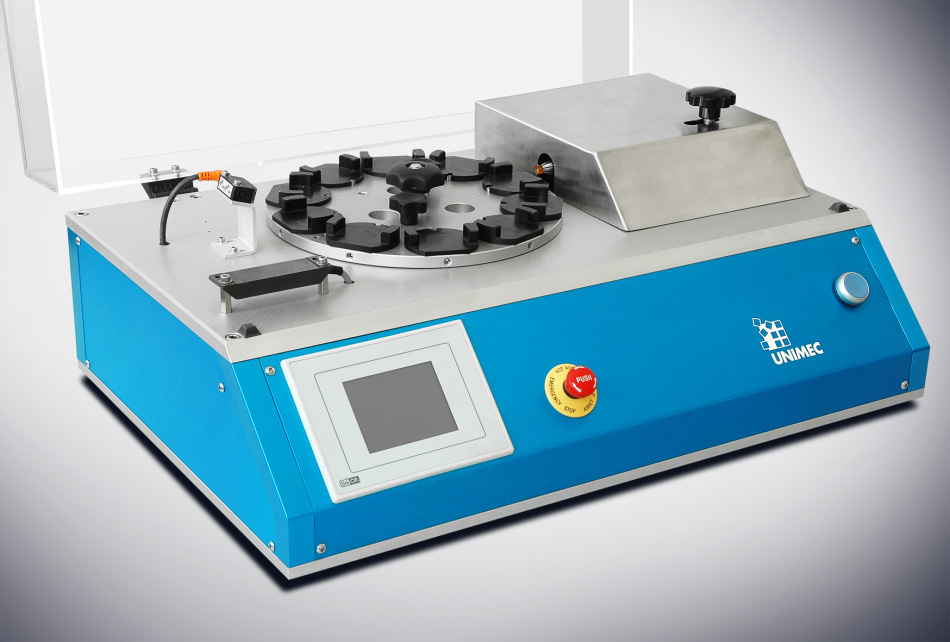
\includegraphics[width=0.49\textwidth]{assets/figures/Etat de l'art/UNIMEC machine complete.jpg}
    \hfill
    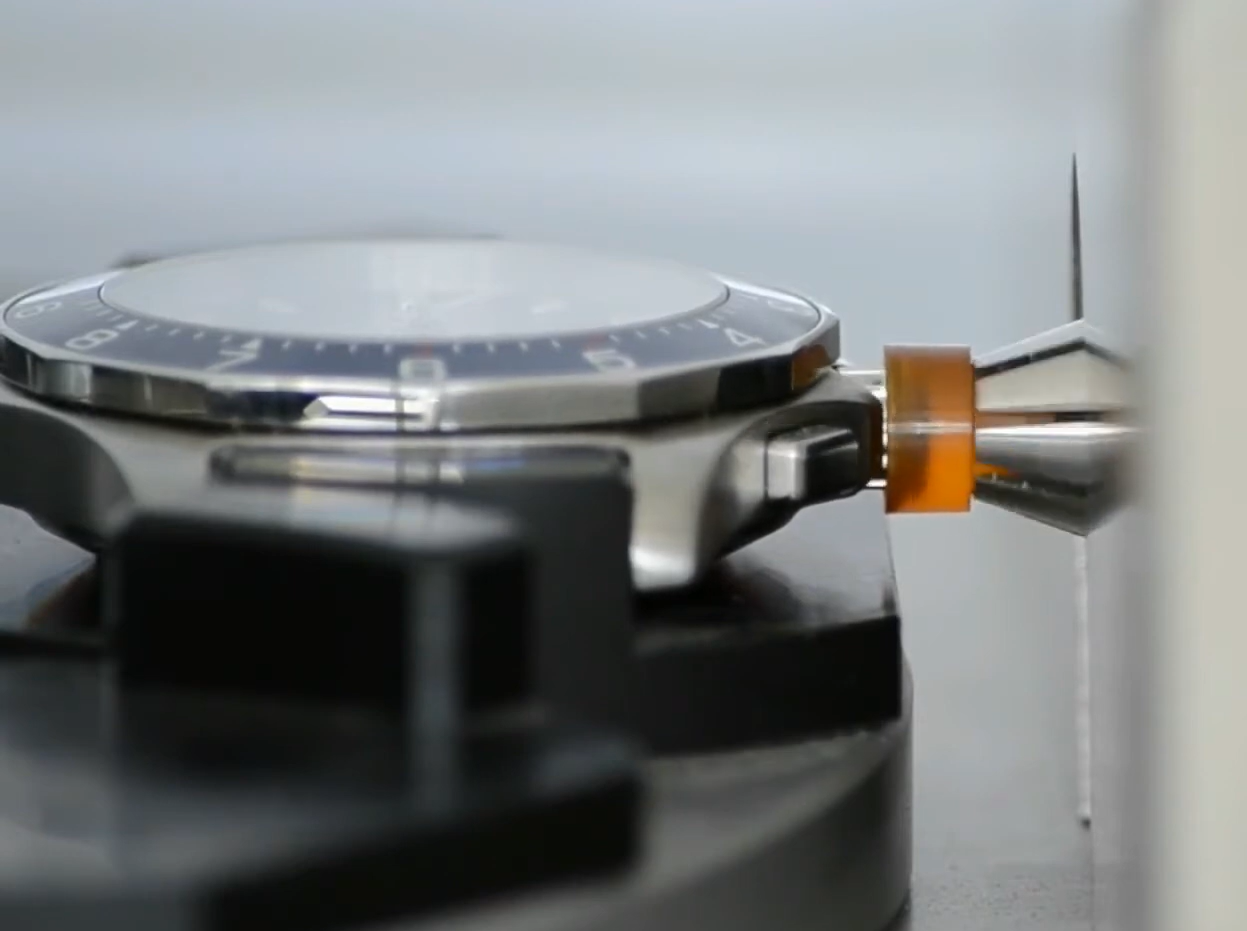
\includegraphics[width=0.49\textwidth]{assets/figures/Etat de l'art/UNIMEC remontage.png}
    \caption{Machine de remontage de montres d'UNIMEC SA \cite{UNIMEC_Remontage}}
    \label{fig:unimec_remontage}
\end{figure}

\subsubsection{Avantages}

La machine de remontage d'UNIMEC SA présente plusieurs avantages significatifs :

\begin{itemize}
    \item \textbf{Automatisation du remontage} : Le remontage automatique permet de standardiser cette étape cruciale du test, éliminant la variabilité introduite par le remontage manuel et garantissant une reproductibilité excellente des conditions initiales.
    
    \item \textbf{Capacité de parallélisation} : La possibilité de remonter simultanément jusqu'à 10 mouvements augmente considérablement la productivité et permet de synchroniser le remontage avec d'autres étapes du processus.
    
    \item \textbf{Système d'embrayage de protection} : L'embrayage de la couronne garantit un remontage sécurisé et non destructif, ce qui est essentiel pour préserver l'intégrité des montres testées.
    
    \item \textbf{Haute flexibilité de programmation} : La capacité à stocker et gérer 31 plateaux programmés différents offre une adaptabilité exceptionnelle à divers types de mouvements et de boîtiers, ce qui est idéal pour les ateliers traitant une grande diversité de modèles.
    
    \item \textbf{Compacité et intégration facile} : Les dimensions réduites (600 × 400 × 240 mm) et la faible consommation électrique (60 W) rendent cet équipement facile à intégrer dans n'importe quel atelier horloger existant.
\end{itemize}

\subsubsection{Inconvénients}

Malgré ses atouts, la machine présente certaines limitations :

\begin{itemize}
    \item \textbf{Fonction limitée au remontage} : Cet équipement est exclusivement dédié au remontage et n'intègre pas d'autres fonctions (mesure de réserve de marche, détection d'arrêt, etc.). Une solution complète de test requiert donc l'intégration avec d'autres appareils ou systèmes.
    
    \item \textbf{Nombre maximal de positions limité à 10} : Bien que cela soit suffisant pour de nombreuses applications, cette limitation peut être un frein pour les environnements de production très haute volume ou pour les ateliers ayant besoin de tester simultanément un grand nombre de modèles différents.
    
    \item \textbf{Absence d'intégration avec la mesure} : La machine ne fournit aucune information ou retour sur l'état du remontage effectué. Une vérification complémentaire est nécessaire pour confirmer que le remontage s'est déroulé correctement, ce qui peut allonger le processus global de test.
\end{itemize}

La machine de remontage d'UNIMEC SA représente une excellente solution pour les ateliers horlogers ayant besoin de remontage automatisé et standardisé. Elle s'intègre naturellement en amont de solutions de mesure complètes telles que le Chronoscope RDM ou le Chrono RMV. La machine proposée dans ce travail pourrait bénéficier d'une intégration conceptuelle avec ce type de remonteur pour offrir une solution de test globale cohérente et efficace.


Les technologies présentées dans cet état de l'art constituent une base de réflexion pour la conception de la machine développée dans ce travail. Le choix final des solutions techniques dépendra des contraintes industrielles, de la précision requise, de la robustesse attendue du système ainsi que de la simplicité d'utilisation pour l'opérateur.
